\normalfont\normalsize
\chapter{Testing}

The tests that we have conducted highlights the strengths of the platform but also reveals some of its weaknesses.

The most important characteristics of this experiment are the maneuverability of the drone with the extra gear, the maximum range of the drone wireless network and the maximum range of the dongle.



\section{Scenario}

The scenario for the test is simple. Using the drone, we must try to connect and collect the data from the nodes.

The testing method were conducted using a dongle with an 8 dBi antenna, a SparrowV3.2  with a standard antenna and a SparrowV3.2 with a 8 dBi antenna, both place on a hill with the antenna directed upwards for a maximum range test. Other  three nodes with 3 dbi external antenna were placed inside of a building. The nodes were configured to send a packet every second The controlling device of the drone was a Samsung Galaxy S4.

Because both the drone and nodes use 2.4 GHz network, the drone was configured to use channel 11 and the nodes to use channel 1 to prevent signal interference.

\begin{figure}[ht]
\begin{center}
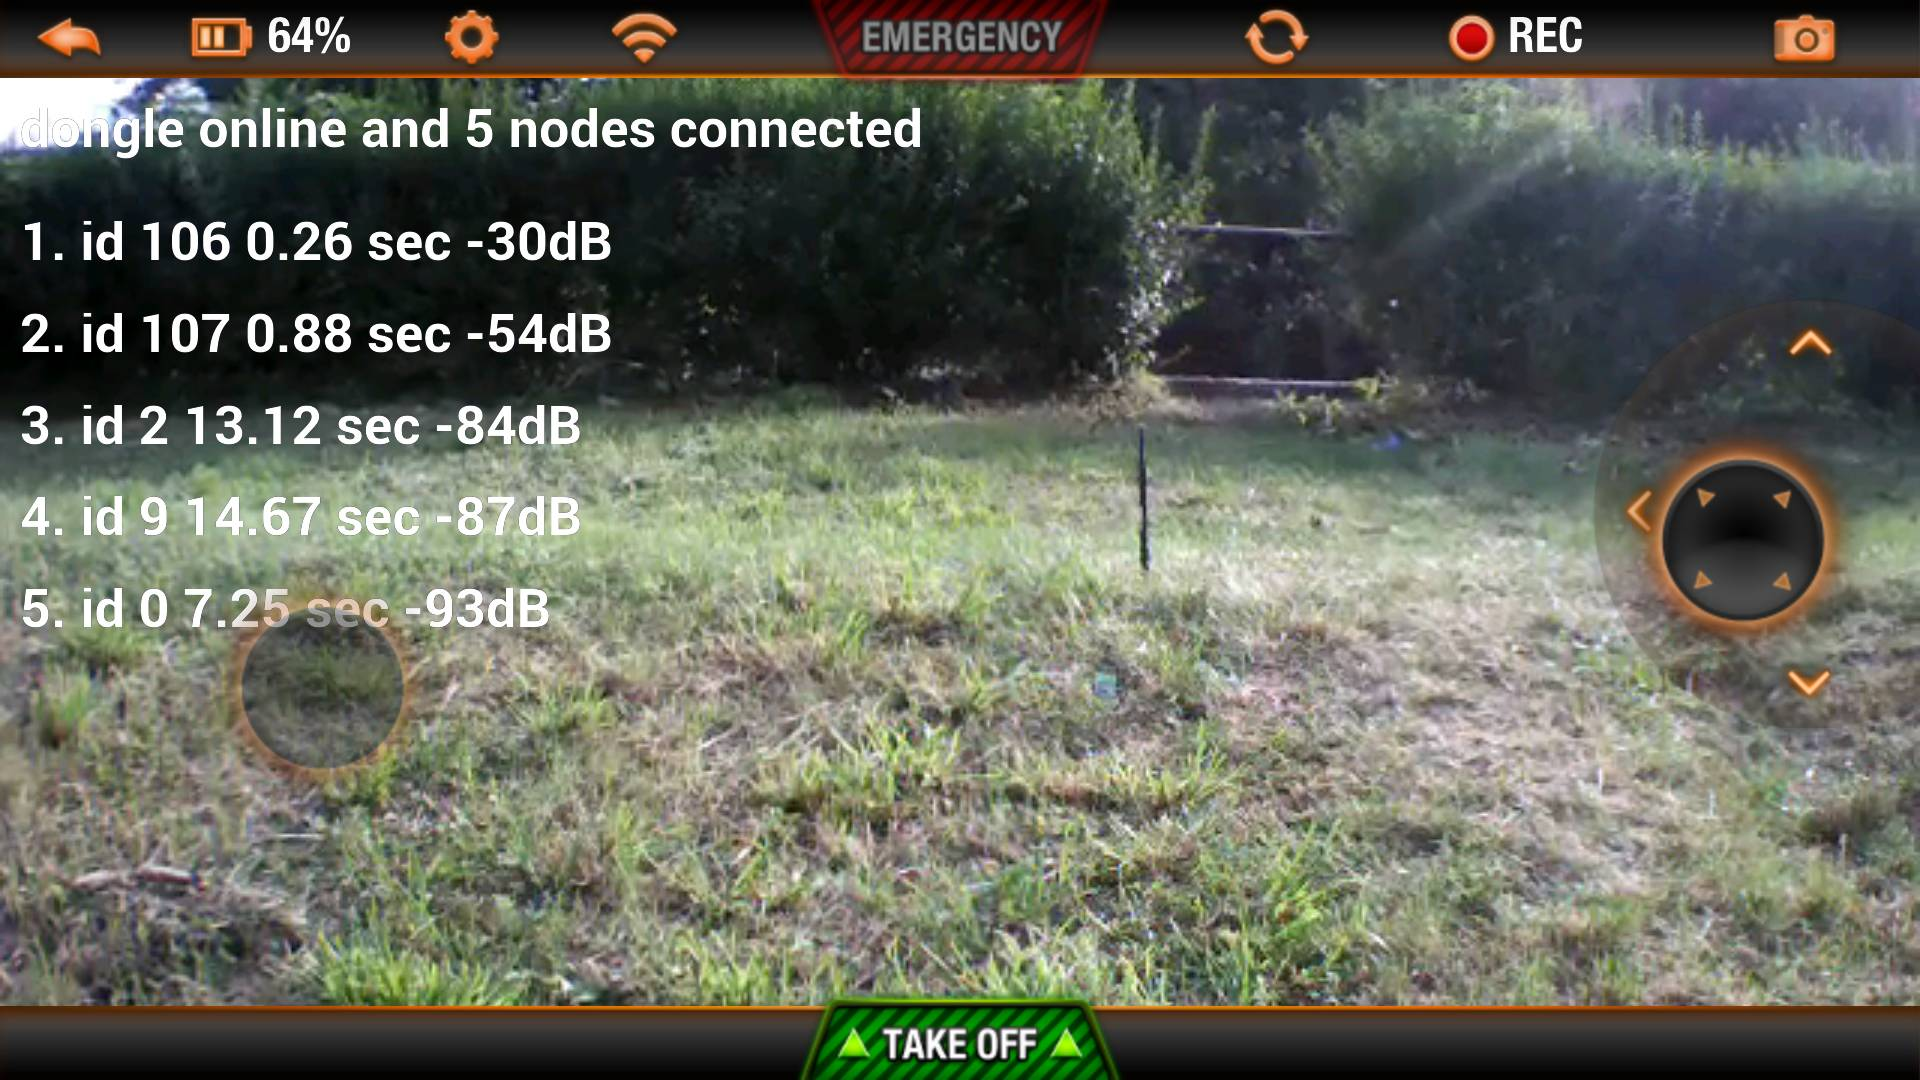
\includegraphics[width=0.9\textwidth]{img/parrot_test.png}
\end{center}
\caption{\small \itshape{Parrot discovering new nodes before takeoff}}
\end{figure}


\section{Results}


\subsection{Signal range}

\begin{figure}[ht]
\begin{center}
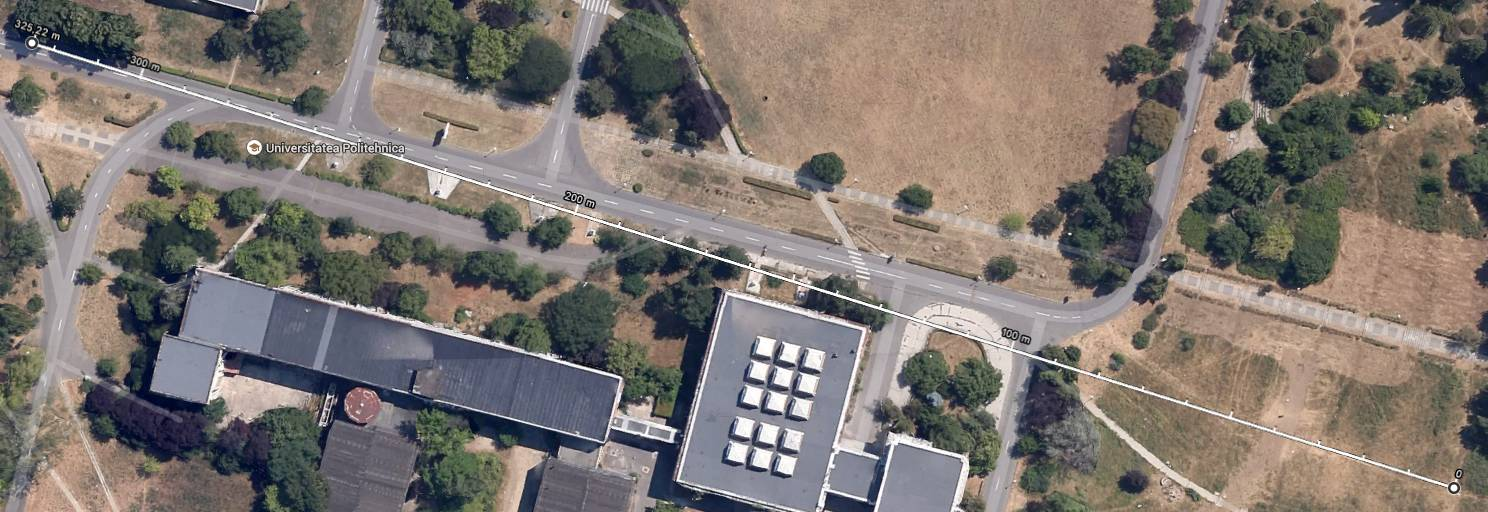
\includegraphics[width=0.9\textwidth]{img/distance.png}
\end{center}
\caption{\small \itshape{Measured signal distance}}
\end{figure}


The drone was able to find the nodes but as expected, the obstructed nodes had a much smaller communication range then the ones placed on the hill. The range test results proved that the drone could receive signal at a maximum distance of 325 meters from the node with the external antenna located on the hill and a clear line of sight. The other node on hill did managed to send data up to 100 meters. In the case of the obstructed nodes, even though they had a 3 dbi antenna, the distance did not exceeded the 50 meters mark. After this distance, the loss of the packets is to big to be able to properly communicate with the nodes, even though occasionally, at 60 meters, some packets were received.


The top mounted antenna worked, but for a better signal, the antenna should always be positioned on the bottom of the drone because in this way, the antenna will have a clear path to send and receive signal and not have the signal blocked by the entire drone and its avionics. The problem with this drone is that on the bottom of it, there are sensors that help it determine the ground speed, ground distance and the antenna, if place on the bottom could obstruct some of the sensors. A vertical antenna will increase the wind resistance an make it too unstable.


\subsection{Drone stability}

Even though the antenna was mounted on top of the parrot, because it is a high gain antenna the signal received is very strong. 

The antenna extended the signal range but also added weight. The dongle is mounted on the side of the drone due to the position of the USB. Because the dongle is not centered on the drone, a counterweight had to be glued on the opposite side on the outer shell to maintain the balance of the drone. 

The drone was relatively stable during the test, but a better stability and flight control could be obtained if the dongle was made smaller and a lighter antenna were mounted.


\begin{figure}[ht]
\begin{center}
\includegraphics[width=0.9\textwidth]{img/parrot_antenna.jpg}
\end{center}
\caption{\small \itshape{Top mounted antenna for better signal}}
\end{figure}

\subsection{Maximum height and maneuverability}

The total added weight is 75 grams. Even though it does not sound that much, it does have a substantial effect on the drone. The maximum height it can reach is 50 meters versus the 75 meters it can reach without the added weight. The maneuverability is also affected, the drone response not being as sharp as before, but it is still good.

\subsection{Problems}

The kernel module needed for the dongle does not recognize the dongle if it is plugged in the drone when it is powered up. The fix is to power up the drone and then plug in the dongle, but this is more difficult then it might appear because every time this action is performed the hull must be repositioned.

\clearpage
